\subsection*{問題1}
電子回路によく使われるコンデンサには,電解コンデンサとセラミックコンデン
サがある.両者の周波数特性とその用途を調べよ.
\begin{description}
    \item[] 電解コンデンサとセラミックコンデンサの周波数特性は図1に示す.また,
    電解コンデンサとセラミックコンデンサの用途は以下のとおりである.
    \begin{itemize}
        \item 電解コンデンサの用途
        \begin{description}
            \item[] 平滑用,デカップリング用
        \end{description}
        \item セラミックコンデンサの用途
        \begin{description}
            \item[] 平滑用,カップリング用,デカップリング用,高周波回路
        \end{description}
    \end{itemize}
\end{description}

\begin{figure}[H]
    \centering
    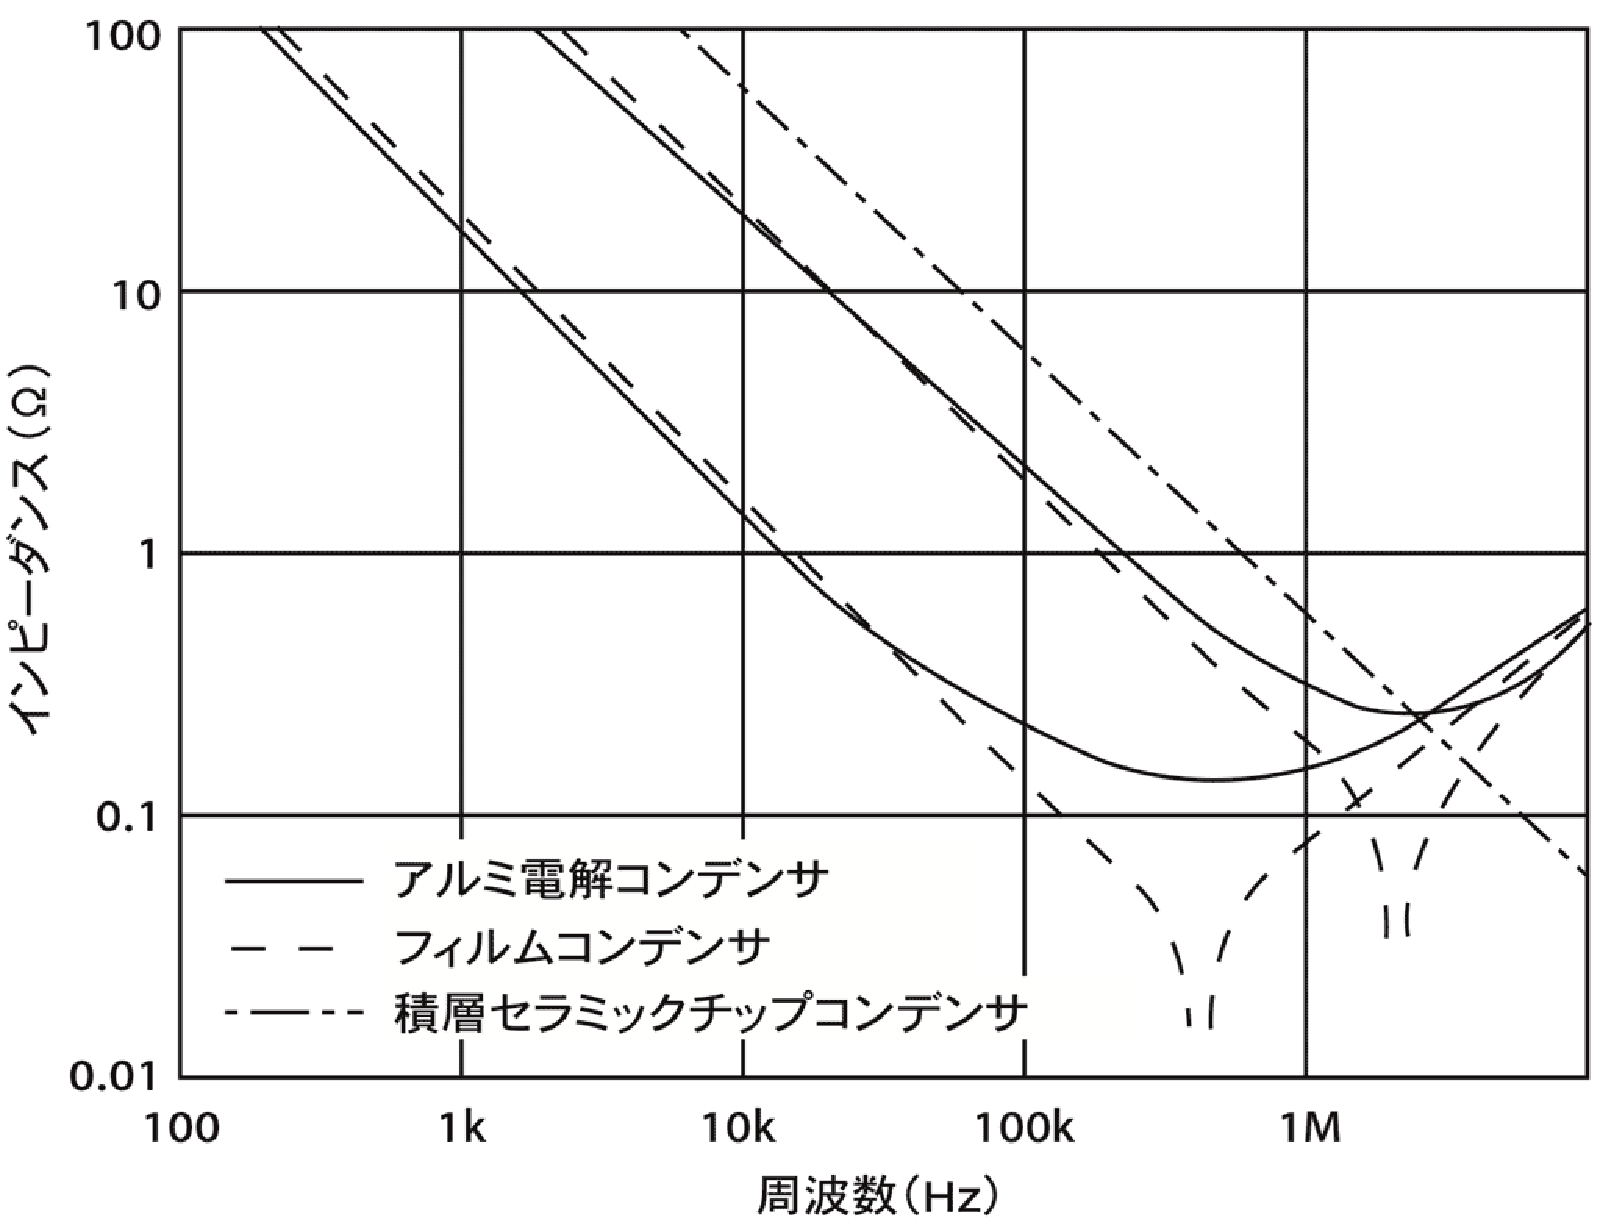
\includegraphics[scale=0.4]{figure1.pdf}
    \caption{電解コンデンサとセラミックコンデンサの周波数特性}
\end{figure}

\subsection*{問題2}
ダイオードの逆方向降伏電圧を用いて一定の電圧を発生するダイオードをな
んと呼ぶか?
\begin{description}
    \item[] ツェナーダイオード
\end{description}

\subsection*{問題3}
LEDには,赤,青,緑等に発光するものがある.色の違いが何によるのか,
青色ダイオードはなぜ最後に発明されたのかを考察せよ.
\begin{itemize}
    \item LEDの色の違いの原因
    \begin{description}
        \item[] 光の波長の違いが,LEDの発光色を決めており,$450\,\si{nm}$前後が青色,
        $520\,\si{nm}$前後が緑色,$660\,\si{nm}$前後が赤色に見える.さらに,
        この光の波長は,Ga(ガリウム),N(窒素),In(インジウム),Al(アルミニウム)
        ,P(リン)など,LEDの半導体を構成する化合物によって決まる.

    \end{description}
    \item 青色ダイオードが最後に開発された原因
    \begin{description}
        \item[] 青色ダイオードの材料となる化合物半導体,窒素ガリウムとサファイアの原子の間隔の差が大きく、
        きれいな結晶を作るのが難しかったためである.結晶の作成に成功した後も,
        ホールを生み出すマグネシウムに,水素原子がくっついて邪魔をしていたために,
        p型のホールがうまく動かなかったために青色ダイオードの発明が難航した.
    \end{description}
\end{itemize}
